% Created 2017-12-14 jeu. 13:46
% Intended LaTeX compiler: pdflatex
\documentclass[10pt,svgnames,fragile]{beamer}

% --- PACKAGES --- %
\usepackage[utf8]{inputenc}
\usepackage[T1]{fontenc}
\usepackage[french]{babel}
\usepackage{csquotes}
\usepackage[toc, page]{appendix}
\usepackage{graphicx}
\usepackage{subcaption}
\usepackage{xcolor}
\usepackage{amsmath, amssymb}
\usepackage{amsthm}
\usepackage{mathrsfs}
\usepackage{booktabs}
\usepackage{float}
\usepackage{setspace}
\usepackage{hyperref}
\usepackage{parskip}
\usepackage{caption}
\usepackage{enumitem}
\usepackage{tikz}
\usepackage{tikz-3dplot}
\usepackage{tkz-tab}
\usepackage{dsfont}

% --- MISE EN PAGES --- %
% itemize avec des points
\setlist[itemize,1]{label={\color{black}\small \textbullet}} 
% permet de numéroter les équations en fonction de la section
\numberwithin{equation}{section}
% pour supprimer l'alinéa
\onehalfspacing

% --- QUELQUES COMMANDES --- %
% Ensembles R et N
\newcommand{\bbR}{\mathbb{R}}
\newcommand{\bbN}{\mathbb{N}}
\newcommand{\bbZ}{\mathbb{Z}}

% Lettres
\newcommand{\calF}{\mathcal{F}}
\newcommand{\calK}{\mathcal{K}}
\newcommand{\calD}{\mathcal{D}}
\newcommand{\calR}{\mathcal{R}}
\newcommand{\calL}{\mathcal{L}}
\newcommand{\calM}{\mathcal{M}}
\newcommand{\calB}{\mathcal{B}}
\newcommand{\calE}{\mathcal{E}}

\newcommand{\scrC}{\mathscr{C}}
\newcommand{\scrS}{\mathscr{S}}
\newcommand{\scrA}{\mathscr{A}}

% Commandes maths
% fonctions vectorielles en gras
\usepackage{bm}
\newcommand{\bfm}[1]{\bm{\mathrm{#1}}}
% divergence
\newcommand{\Div}{\mathrm{div}}
% produit scalaire
\newcommand{\ps}[2]{\langle #1, #2 \rangle}
% norme
\newcommand{\norm}[1]{\left\lVert #1 \right\rVert}
% Commande norme triple
\newcommand{\vertiii}[1]{{\left\vert\kern-0.25ex\left\vert
    \kern-0.25ex\left\vert #1 
\right\vert\kern-0.25ex\right\vert\kern-0.25ex\right\vert}}
% valeur absolue
\newcommand{\abs}[1]{\displaystyle\left\lvert #1 \right\rvert}
% exponentielle
\newcommand{\ex}{\mathrm{e}}
% H^1_0(Omega)
\newcommand{\Hone}[1][\Omega]{H^1_0(#1)}
% D(Omega)
\newcommand{\scrD}{\mathscr{D}(\Omega)}
% opérateurs
\newcommand{\operateurs}{M^{-1}_0 L_0}
% limite
\newcommand{\limm}{\underset{h \rightarrow0}{\lim} \ \dfrac{1}{h}}
% ensemble des fonctions à croissances au plus polynomiales
\newcommand{\scrCinfp}{\scrC^{\infty}_p}

% --- NUMEROTATION THEOREMES --- % 
\newtheorem{theoreme}{Théorème}[section]
\newtheorem{proposition}{Proposition}[section]
\newtheorem{remark}{Remarque}[section]


\usepackage{etex}
\usepackage[normalem]{ulem}
\usepackage{textcomp}
\usepackage{pdflscape}
\usepackage{marvosym}
\usepackage{wasysym}
\usepackage{qtree}
\usepackage{bussproofs}
\usepackage{proof}
\usepackage{fitch}
\usepackage{cancel}
\usepackage{url}
\usepackage{smfthm}

%% le code qui suit permet le rappel du plan à chaque changement de section:
\AtBeginSection[]{
  \begin{frame}
    \footnotesize\tableofcontents[sectionstyle=show/shaded, subsectionstyle=show/show/shaded]
  \end{frame}
}

\AtBeginSubsection[]{
  \begin{frame}
    \footnotesize\tableofcontents[sectionstyle=show/shaded, subsectionstyle=show/shaded/shaded]
  \end{frame}
}
\subtitle{}

\titlegraphic{
\includegraphics[height=2.5cm]{images/logo_um.png} \hspace{1cm} 
\includegraphics[height=2cm]{images/logo_dpt_maths.png}}

\institute[]{} \usetheme{CambridgeUS}
\usepackage{beamer_udl_theme}
\setbeamertemplate{navigation symbols}{%
	%insertslidenavigationsymbol%
	%insertframenavigationsymbol%
	%insertsubsectionnavigationsymbol%
	%insertsectionnavigationsymbol%
	%insertdocnavigationsymbol%
	%insertbackfindforwardnavigationsymbol%
}

\setbeamertemplate{section in toc}{%
  \inserttocsectionnumber.~\inserttocsection
}
\setbeamertemplate{subsection in toc}{%
  \hspace{1.5em}\inserttocsectionnumber.\inserttocsubsectionnumber~\inserttocsubsection\par
}

\usetheme{default}
\author{Hugo JOHNSON \& Quentin LAHAYE}
\date{}
\title{Autour de l'équation de Rayleigh-Stokes}

\begin{document}

\maketitle

\begin{frame}{Introduction}
L'équation de Rayleigh-Stokes est une équation aux dérivées 
partielles utilisée en dynamique des fluides pour modéliser le 
comportement des 
fluides de second grade. Une forme canonique de l'équation pour 
une fonction de vitesse $u$ est
\begin{equation*}
    \partial_t u - \nu \Delta u - \alpha \Delta \big(\partial_t u\big) = f
\end{equation*}
%où
%\begin{itemize}
%   \item $\nu$ est la viscosité cinématique du fluide, responsable de la diffusion classique,
%   \item $\alpha$ est le paramètre de Rayleigh-Stokes, lié aux propriétés viscoélastiques du fluide,
%   \item $f$ est un terme de forçage,
%   \item $\Delta \big(\partial_t u\big)$ est un terme dit de \og dispersion régularisée \fg{} qui caractérise le comportement du fluide sous l'effet d'une accélération.
%\end{itemize}
\end{frame}

\footnotesize\tableofcontents

\section{Le premier problème de Stokes}
\begin{frame}
\begin{itemize}
    \item On considère un fluide visqueux au repos que l'on suppose incompressible, 
homogène et ne subissant aucune force extérieure. Le problème de Stokes consiste à étudier 
la vitesse du fluide dans la situation suivante
\end{itemize}
\begin{figure}[!h]
    \centering
    \tdplotsetmaincoords{70}{120}
    \begin{tikzpicture}[tdplot_main_coords, scale=1.4]
        % ----- PLAQUE (plan y=0, dans le plan xz) -----
        \fill[blue!15, opacity=0.7] (-2.5,-2.5,0) -- (2.5,-2.5,0) -- (2.5,2.5,0) -- (-2.5,2.5,0) -- cycle;
        \draw[gray!60] (-2.5,-2.5,0) -- (2.5,-2.5,0) -- (2.5,2.5,0) -- (-2.5,2.5,0) -- cycle;
        % Label plaque
        \node[blue!60!black] at (2.8, 1.5, 0) {plaque $y=0$};

        % ----- REPÈRE -----
        % Axe x (e1)
        \draw[->, thick] (0,0,0) -- (2.5,0,0) node[anchor=north] {$x$};
        \draw[->, red] (0,0,0) -- (1,0,0) node[above left] {$e_1$};
        % Axe y (e2) vers le haut
        \draw[->, thick] (0,0,0) -- (0,0,2.5) node[anchor=south] {$y$};
        \draw[->, green] (0,0,0) -- (0,0,1) node[right] {$e_2$};
        % Axe z (e3)
        \draw[->, thick] (0,0,0) -- (0,2.5,0) node[anchor=west] {$z$};
        \draw[->, blue] (0,0,0) -- (0,1,0) node[below right] {$e_3$};
        % Origine
        \filldraw[black] (0,0,0) circle (1.5pt) node[below] {$O$};

        % ----- FLUIDE (demi-espace y>0) -----
        \fill[cyan!10, opacity=0.3]
            (-2.5,-2.5,0) -- (2.5,-2.5,0) -- (2.5,-2.5,2.2)
            -- (-2.5,-2.5,2.2) -- cycle;
        \fill[cyan!10, opacity=0.3]
            (2.5,-2.5,0) -- (2.5,2.5,0) -- (2.5,2.5,2.2)
            -- (2.5,-2.5,2.2) -- cycle;
        \fill[cyan!10, opacity=0.3]
            (-2.5,-2.5,2.2) -- (2.5,-2.5,2.2) -- (2.5,2.5,2.2)
            -- (-2.5,2.5,2.2) -- cycle;
        \fill[cyan!10, opacity=0.3]
            (2.5,2.5,0) -- (-2.5,2.5,0) -- (-2.5,2.5,2.2)
            -- (2.5,2.5,2.2) -- cycle;
        \node[cyan!50!black] at (2.2, -1.5, 1.8) {fluide $y>0$};

        % ----- FLÈCHE DE DÉPLACEMENT DE LA PLAQUE -----
        \draw[->, line width=2pt, red!80!black]
            (-0.5, -1.8, 0) -- (1.2, -1.8, 0)
            node[midway, above, sloped] {\small $V e_1$};

        % ----- POINT X -----
        \filldraw[black] (-0.4, 1.0, 1.2) circle (1.5pt);
        \node[above right] at (-0.4, 1.0, 1.2) {$X = (x,y,z)$};
    \end{tikzpicture}
    \caption{Configuration du premier problème de Stokes}
    \label{fig:pbmStokes}
\end{figure}
\end{frame}

\begin{frame}
\begin{itemize}
\item On considère donc la vitesse du fluide
\begin{eqnarray*}
    \bfm{u} : \bbR^3 \times \bbR_+ \longrightarrow \bbR^3, \
    (X,t) \longmapsto \big(u_1(X,t), u_2(X,t), u_3(X,t)\big)
\end{eqnarray*} 
\item Le contexte du premier problème de Stokes nous amène à quelques 
simplifications. 
\begin{equation*}
    \bfm{u} (X,t) = \big(u_1(y,t),0,0\big)
\end{equation*} 
\item Comme le fluide est incompressible et homogène on a 
\begin{eqnarray*}
    \rho(X,t) \equiv \rho > 0 \ \ \ &\text{ et }& \ \ \ \Div(\bfm{u})=0
\end{eqnarray*} 
\item Les équations du mouvement du milieu continu nous donne 
\begin{equation}\label{PFD1}
    \rho \frac{D\bfm{u}}{Dt} = \Div(\sigma) + \rho \bfm{f}
\end{equation}
\end{itemize}
\end{frame}

\begin{frame}
\begin{itemize}
    \item Pour un fluide de second grade, le tenseur des contraintes est 
donné par le théorème de Rivlin-Ericksen 
\begin{equation*}
    \sigma := -pI + \mu A_1 + \alpha_1 A_2 + \alpha_2 A_1^2
\end{equation*}
où
\begin{itemize}
    \item[$\triangleright$] $pI$ est la contrainte isotropique avec $p$ la pression,
    \item[$\triangleright$] $A_1 := \nabla \bfm{u} + \nabla^t \bfm{u}$,
    \item[$\triangleright$] $A_2 := \dfrac{D}{Dt}A_1 + A_1\nabla \bfm{u} + \nabla^t\bfm{u} A_1$,
    \item[$\triangleright$] $\mu >0$ est la viscosité du fluide,
    \item[$\triangleright$] $\alpha_1$ et $\alpha_2$ sont des paramètres thermodynamiques qui doivent vérifier 
    \begin{eqnarray*}
        \alpha_1 \geq 0 \ \ \ \ \ \text{ et } \ \ \ \ \ \alpha_1 + \alpha_2 = 0
    \end{eqnarray*}
    pour que le modèle soit physiquement admissible.
\end{itemize}
\end{itemize}
\end{frame}

\begin{frame}
\begin{itemize}
    \item Le tenseur des contraintes est
\begin{equation*}
    \sigma = \begin{pmatrix}
        -p+\alpha_2(\partial_yu_1)^2 & \mu\partial_yu_1 + \alpha_1 \partial_{ty}u_1 & 0 \\
        \mu \partial_yu_1+\alpha_1\partial_{ty} u_1 & -p+(2\alpha_1+\alpha_2)(\partial_yu_1)^2 & 0 \\
        0 & 0 & -p
    \end{pmatrix}
\end{equation*} 
\item On applique l'opérateur divergence à $\sigma$ et on injecte dans \eqref{PFD1} et 
\begin{equation*}
    \left\{\begin{array}{rcl}
        \rho\partial_tu_1 & = & -\partial_xp + \mu \partial_{yy}u_1 + \alpha_1 \partial_{yty}u_1  \\
        0 & = & - \partial_yp+2(2\alpha_1+\alpha_2)\partial_yu_1\partial_{yy}u_1 \\
        0 & = & - \partial_zp
    \end{array}\right.
\end{equation*}
    \item L'invariance par translation dans les directions $e_1$ et $e_3$ implique que 
la pression ne dépend pas de $x$ et $z$, donc $\partial_xp=0$.
\item On obtient finalement l'équation de Rayleigh-Stokes homogène en une dimension
\begin{equation*}
    \partial_t u_1 - \nu \partial_{yy}u_1 - \alpha \partial_{tyy}u_1=0
\end{equation*}
où $\nu := \dfrac{\mu}{\rho}$ et $\alpha := \dfrac{\alpha_1}{\rho}$.
\end{itemize}
\end{frame}

%\begin{frame}
%\begin{itemize}
%    \item L'invariance par translation dans les directions $e_1$ et $e_3$ implique que 
%la pression ne dépend pas de $x$ et $z$, donc $\partial_xp=0$.
%\item On obtient finalement l'équation de Rayleigh-Stokes homogène en une dimension
%\begin{equation*}
%    \partial_t u_1 - \nu \partial_{yy}u_1 - \alpha \partial_{tyy}u_1=0
%\end{equation*}
%où $\nu := \dfrac{\mu}{\rho}$ et $\alpha := \dfrac{\alpha_1}{\rho}$.
%\end{itemize}
%\end{frame}

\section{Analyse de Fourier}
\begin{frame}
    On considère le problème
\begin{equation*}
    \begin{cases}
        \partial_tu(t,x) - \nu\Delta u(t,x) - \alpha\Delta \big(\partial_t u(t,x)\big) = 0 & (t,x) \in \mathbb R_+ \times \bbR^d  \\
        u(0,x) = u_0(x) & x \in \bbR^d
    \end{cases}
\end{equation*}
\end{frame}

\subsection{Donnée initiale dans \texorpdfstring{$\scrS'(\bbR^d)$}{S'(Rd)}}
\begin{frame}{Unicité}
\begin{itemize}
\item On considère $u_0 \in \scrS'(\bbR^d)$. On peut reformuler le 
problème précédent de la façon suivante : trouver $u \in 
\scrC^1(\bbR_+, \scrS'(\bbR^d))$ tel que
\begin{equation}\label{pb_RS4}
    \begin{cases}
        u'(t) - \nu\Delta u(t) - \alpha\Delta \big(u'(t)\big) = 0  \\
        u(0) = u_0
    \end{cases}
\end{equation}
\item On suppose qu'il existe une solution 
$u \in \scrC^1(\bbR_+,\scrS'(\bbR^d))$. On applique la 
transformée de Fourier au problème.% \eqref{pb_RS4}.
%\begin{equation*}
%    \calF\big(u'(t)\big)-\nu\calF\big(\Delta u(t)\big)-\alpha\calF\big(\Delta(u'(t))\big) = 0
%\end{equation*} 
%\item On montre que $\calF\big(u'(t)\big)=\hat{u}'(t)$ et  que $\calF\Big(\dfrac{\mathrm{d}}{\mathrm{d}t}\Delta u(t)\Big) 
%= -\|\xi\|^2\hat{u}'(t)$. 
\item On obtient le problème suivant
\begin{equation}\label{pb_RS_Fourier}
    \begin{cases}
        (1+\alpha\|\xi\|^2)\hat{u}'(t)+\nu\|\xi\|^2\hat{u}(t) = 0  \\
        \hat{u}(0) = \hat{u}_0
    \end{cases}
\end{equation}
\end{itemize}
\end{frame}

%\begin{frame}{Unicité}
%    \begin{itemize}
%\item On suppose qu'il existe une solution 
%$u \in \scrC^1(\bbR_+,\scrS'(\bbR^d))$. On applique la 
%transformée de Fourier au problème \eqref{pb_RS4}.
%\begin{equation*}
%    \calF\big(u'(t)\big)-\nu\calF\big(\Delta u(t)\big)-\alpha\calF\big(\Delta(u'(t))\big) = 0
%\end{equation*} 
%\item On montre que $\calF\big(u'(t)\big)=\hat{u}'(t)$ et  que $\calF\Big(\dfrac{\mathrm{d}}{\mathrm{d}t}\Delta u(t)\Big) 
%= -\|\xi\|^2\hat{u}'(t)$. 
%\item Finalement, on obtient le problème suivant
%\begin{equation}\label{pb_RS_Fourier}
%    \begin{cases}
%        (1+\alpha\|\xi\|^2)\hat{u}'(t)+\nu\|\xi\|^2\hat{u}(t) = 0  \\
%        \hat{u}(0) = \hat{u}_0
%    \end{cases}
%\end{equation}
%\end{itemize}
%\end{frame}

\begin{frame}{Unicité}
\begin{itemize}
    \item Donc 
\begin{equation*}
    \hat{u}(t)(\xi) = \exp\bigg(\frac{-\nu \|\xi\|^2}{1+\alpha\|\xi\|^2}t\bigg)\hat{u}_0(\xi)
\end{equation*} 
\item On pose alors 
\begin{equation}\label{sol_Fourier}
    \forall (t,x) \in \bbR_+\times \bbR^d, \ u(t,\xi) = \calF^{-1}\bigg(\exp\bigg(\frac{-\nu \|\xi\|^2}{1+\alpha\|\xi\|^2}t\bigg)\hat{u}_0(\xi)\bigg)(x)
\end{equation}
Ce qui démontre l'unicité de la solution de \eqref{pb_RS4}.
\end{itemize}
\end{frame}

\begin{frame}{Existence}
\begin{itemize}
\item On va maintenant montrer que $u$ définie 
par \eqref{sol_Fourier} est solution de classe $\scrC^1$ de 
\eqref{pb_RS4}. 
\item On pose 
\begin{equation*}
    \forall (t,\xi) \in \bbR_+ \times \bbR^d, \ \hat{\calK}(t,\xi) := \exp\Big(\dfrac{-\nu \|\xi\|^2}{1+\alpha\|\xi\|^2}t\Big)
\end{equation*} 
\item Le fait que $\hat{\calK}(t,\cdot)$ soit un multiplicateur de 
$\scrS'(\bbR^d)$ nous permet de montrer que $\hat{u}$ est 
dérivable et que $\hat{u}'$ est continue.
    \item On vérifie aisément que 
\begin{equation*}
    \hat{u}(0)=\hat{u}_0
\end{equation*}
et que $\hat{u}(t)$ est solution de \eqref{pb_RS_Fourier} pour 
tout $t \in \bbR_+$. 
\item En utilisant les propriétés de $\calF$, on en déduit que \eqref{sol_Fourier} est 
solution de \eqref{pb_RS4} pour tout $t \in \bbR_+$. 
\item Enfin, en 
utilisant la formule d'inversion de Fourier et le lien entre 
convolution et transformée de Fourier, on peut réécrire l'expression de la 
solution
\begin{eqnarray}\label{sol_S'}
     u(t,x) = \frac{1}{(2\pi)^{d/2}}K(t,x)*u_0(x)
\end{eqnarray}
\end{itemize}
\end{frame}

%\begin{frame}{Existence}
%    \begin{itemize}
%    \item On vérifie aisément que 
%\begin{equation*}
%    \hat{u}(0)=\hat{u}_0
%\end{equation*}
%et que $\hat{u}(t)$ est solution de \eqref{pb_RS_Fourier} pour 
%tout $t \in \bbR_+$. 
%\item En utilisant les propriétés de $\calF$, on en déduit que \eqref{sol_Fourier} est 
%solution de \eqref{pb_RS4} pour tout $t \in \bbR_+$. 
%\item Enfin, en 
%utilisant la formule d'inversion de Fourier et le lien entre 
%convolution et transformée de Fourier, on peut réécrire l'expression de la 
%solution
%\begin{eqnarray}\label{sol_S'}
%     u(t,x) = \frac{1}{(2\pi)^{d/2}}K(t,x)*u_0(x)
%\end{eqnarray}
%\end{itemize}
%\end{frame}

\subsection{Donnée initiale dans \texorpdfstring{$H^s(\bbR^d)$}{Hs(Rd)}}

\begin{frame}
\begin{itemize}
\item On considère maintenant $u_0 \in H^s(\bbR^d)$. Comme 
$H^s(\bbR^d) \subset \scrS'(\bbR^d)$, on peut utiliser les 
résultats de la partie précédente qui nous assure de l'existence 
d'une solution dans $\scrS'(\bbR^d)$. 
\item Il suffit donc de montrer 
que la solution définie par \eqref{sol_S'} est dans 
$\scrC^1(\bbR_+,H^s(\bbR^d))$ ce qui nous donnera l'unicité de 
la solution dans $H^s(\bbR^d)$.
    \item Comme $\calF$ réalise une isométrie entre $H^s(\bbR^d)$ et 
$L^2_s(\bbR^d)$, on a
\begin{eqnarray*}
    u \in \scrC^1(\bbR_+,H^s(\bbR^d)) &\iff& \hat{u} \in \scrC^1(\bbR_+, L^2_s(\bbR^d))
\end{eqnarray*} 
\item Comme $u_0 \in H^s(\bbR^d)$, $\hat{u}_0 \in L_s^2(\bbR^d)$ donc pour presque tout $\xi \in \bbR^d$, $t \mapsto \hat{u}(t,\xi)$ est continue. On a également
\begin{equation*}
    \sup_{t \in \bbR_+}|\hat{u}(t,\cdot)| \leq |\hat{\calK}(t,\cdot)||\hat{u}_0| \leq |\hat{u}_0| \in L^2_s(\bbR^d)
\end{equation*} 
\item Enfin, 
\begin{equation*}
    \sup_{t \in \bbR_+} |\hat{u}'(t)| \leq \frac{\nu\|\xi\|^2}{1+\alpha\|\xi\|^2}|\hat{\calK}(t,\cdot)||\hat{u}_0| \leq \frac{\nu}{\alpha}|\hat{u}_0| \in L^2_s(\bbR^d)
\end{equation*}
Ce qui nous assure par théorème de convergence dominée que $\hat{u} \in \scrC^1(\bbR_+,L^2_s(\bbR^d))$.
\item Donc \eqref{sol_S'} avec $u_0 \in H^s(\bbR^d)$ est solution dans $H^s(\bbR^d)$.
\end{itemize}
\end{frame}

%\begin{frame}
%    \begin{itemize}
%    \item Comme $\calF$ réalise une isométrie entre $H^s(\bbR^d)$ et 
%$L^2_s(\bbR^d)$, on a
%\begin{eqnarray*}
%    u \in \scrC^1(\bbR_+,H^s(\bbR^d)) &\iff& \hat{u} \in \scrC^1(\bbR_+, L^2_s(\bbR^d))
%\end{eqnarray*} 
%\item Comme $u_0 \in H^s(\bbR^d)$, $\hat{u}_0 \in L_s^2(\bbR^d)$ donc pour presque tout $\xi \in \bbR^d$, $t \mapsto \hat{u}(t,\xi)$ est continue. On a également
%\begin{equation*}
%    \sup_{t \in \bbR_+}|\hat{u}(t,\cdot)| \leq |\hat{\calK}(t,\cdot)||\hat{u}_0| \leq |\hat{u}_0| \in L^2_s(\bbR^d)
%\end{equation*} 
%\item Enfin, 
%\begin{equation*}
%    \sup_{t \in \bbR_+} |\hat{u}'(t)| \leq \frac{\nu\|\xi\|^2}{1+\alpha\|\xi\|^2}|\hat{\calK}(t,\cdot)||\hat{u}_0| \leq \frac{\nu}{\alpha}|\hat{u}_0| \in L^2_s(\bbR^d)
%\end{equation*}
%Ce qui nous assure par théorème de convergence dominée que $\hat{u} \in \scrC^1(\bbR_+,L^2_s(\bbR^d))$.
%\item Donc \eqref{sol_S'} avec $u_0 \in H^s(\bbR^d)$ est solution dans $H^s(\bbR^d)$.
%\end{itemize}
%\end{frame}

\subsection{Comportement de la solution et comparaison avec l'équation de la chaleur}

\begin{frame}
    On rappelle l'équation de la chaleur
\begin{equation*}
    \begin{cases}
        \partial_tv(t,x)-\nu\Delta v(t,x)=0 & (t,x) \in \bbR_+ \times \bbR^d \\
        v(0,x) = v_0(x) & x \in \bbR^d
    \end{cases}
\end{equation*}
dont la solution est donnée par 
\begin{equation*}
    \forall (t,x) \in \bbR_+ \times \bbR^d, \ v(t,x) = \calF^{-1}\big(\exp(-\nu t\|\xi\|^2\big)\hat{v}_0(\xi)\big)(x)
\end{equation*}
\end{frame}

\begin{frame}
\begin{itemize}
    \item Dans un premier temps, on raisonne à $t \in \bbR_+$ fixé.
    \item A hautes fréquences, on remarque qu'on a l'équivalent suivant
    \begin{eqnarray*}
        \hat{\calK}(t,\xi) &\underset{\|\xi\|\to+\infty}{\sim}& \exp\Big(-\frac{\nu}{\alpha}t\Big)
    \end{eqnarray*}
    Donc le noyau $\hat{\calK}$ agit comme une multiplication par un scalaire. Donc
    \begin{eqnarray*}
        \hat{u}(t,\xi) &\underset{\|\xi\|\to+\infty}{\sim}& \exp\Big(-\frac{\nu}{\alpha}t\Big)\hat{u}_0(\xi)
    \end{eqnarray*}
        \item A basses fréquences, on peut effectuer un développement limité qui nous amène à
    \begin{eqnarray*}
        \hat{\calK}(t,\xi) &\underset{\|\xi\|\to 0}{\sim}& \exp(-\nu\|\xi\|^2t)
    \end{eqnarray*}
    Donc on a 
    \begin{eqnarray*}
        \hat{u}(t,\xi) &\underset{\|\xi\|\to 0}{\sim}& \exp(-\nu\|\xi\|^2t)\hat{u}_0(\xi)
    \end{eqnarray*}
\end{itemize}
\end{frame}

\begin{frame}
    \begin{itemize}
    \item Maintenant, si on regarde quand $t \to +\infty$ alors à hautes fréquences, comme on a l'équivalent
\begin{eqnarray*}
    \hat{\calK}(t,\xi) &\underset{\|\xi\|\to+\infty}{\sim}& \exp\Big(-\frac{\nu}{\alpha}t\Big)
\end{eqnarray*}
le noyau $\hat{\calK}$ va décroître de manière exponentielle. 
\item Tandis qu'à basses fréquences, 
\begin{eqnarray*}
    \hat{\calK}(t,\xi) &\underset{\|\xi\|\to 0}{\sim}& \exp(-\nu\|\xi\|^2t)
\end{eqnarray*}
donc le noyau $\hat{\calK}$ décroît plus lentement.
    \item La dynamique de la solution est donc dominée par les basses fréquences. On en déduit l'équivalent de la solution en temps long
\begin{eqnarray*}
    \hat{u}(t,\xi) &\underset{t \to +\infty}{\sim}& \exp(-\nu\|\xi\|^2t)\hat{u}_0(\xi)
\end{eqnarray*} 
\item Donc en temps long, la solution de l'équation de Rayleigh-Stokes se comporte comme la solution de l'équation de la chaleur.
\end{itemize}
\end{frame}

%\begin{frame}[label={sec:org9c62e72}]{}
%\begin{block}{Titre et texte encadré}
%Du texte et encore du texte\ldots{} 
%\end{block}
%\end{frame}

\section{Approche variationnelle}
\begin{frame}
    \begin{itemize}
        \item     Soit $d \in \bbN^*$. Soit un ouvert borné $\Omega \subset \bbR^d$.
Pour simplifier l'étude, on prendra des conditions de Dirichlet homogènes et un second membre nul.
Si on se donne une donnée initiale $u_0$, on peut reformuler 
l'équation de Rayleigh-Stokes de la façon suivante : trouver $u \in \scrC^1(\bbR, \Hone)$ 
tel que pour tout $t \in \bbR$
\begin{equation}\label{pb_RS}
\begin{cases}
    u'(t) - \nu\Delta u(t) - \alpha\Delta \big(u'(t)\big) = 0  \\
    u(0) = u_0
\end{cases}
\end{equation}
\item     On définit deux opérateurs $M$ et $L$ par
\begin{eqnarray*}
    M := I - \alpha \Delta \ \ \ \ \ &\text{ et }& \ \ \ \ \ L :=-\nu\Delta
\end{eqnarray*}
de sorte à reformuler le problème \eqref{pb_RS} en : trouver $u \in \scrC^1(\bbR, \Hone)$ tel que pour tout $t \in \bbR$
\begin{equation}\label{RS_forme_operateur}
\begin{cases}
    Mu'(t) + Lu(t)=0  \\
    u(0) = u_0
\end{cases}
\end{equation} 
    \end{itemize}
\end{frame}

\subsection{Extension de $M$ et $L$}

\begin{frame}
\begin{block}{Théorème}
    Soient $(H, \langle \cdot, \cdot \rangle)$ et $(H_0, \langle \cdot, \cdot \rangle_0)$ deux espaces de Hilbert tels que $H$ est un sous-espace dense de $H_0$ et 
\begin{equation}\label{ineq_thm_lax}
    \exists k >0,\ \forall x \in H, \ \norm{x} \geq k \norm{x}_0
\end{equation}
Soit $B$ une forme bilinéaire continue et coercive sur $H$. Alors il existe deux opérateurs linéaires $E$ et $E^*$, dont les domaines de définitions $D$ et $D^*$ sont denses dans $H$, tels que
\begin{enumerate}
    \item[1.] On a
    \begin{eqnarray*}
        \forall x \in D,\ \forall y \in H, \ B(x,y) &=& \ps{Ex}{y}_0 \\
        \forall y \in D^*,\ \forall x \in H, \ B(x,y) &=& \ps{x}{E^* y}_0
    \end{eqnarray*}
    \item[2.] L'image de $E$ est $H_0$, de même pour $E^*$.
    \item[3.] $E$ et $E^*$ admettent des inverses $S$ et $S^*$ qui sont continus de $H_0$ dans $H$.
    \begin{eqnarray*}
        \exists k_1>0,\ \forall z \in H_0, \ \norm{Sz} &\leq& k_1 \norm{z}_0 \\
        \exists k_1^*>0,\ \forall z \in H_0, \ \norm{S^*z} &\leq& k_1^* \norm{z}_0
    \end{eqnarray*}
    Et donc, avec \eqref{ineq_thm_lax}, $S$ et $S^*$ sont continus de $H_0$ dans $H_0$
    %\begin{eqnarray*}
    %    \exists k_2>0,\ \forall z \in H_0, \ \norm{Sz}_0 &\leq& k_2 \norm{z}_0 \\
    %    \exists k_2^*>0,\ \forall z \in H_0, \ \norm{S^*z}_0 &\leq& k_2^* \norm{z}_0
    %\end{eqnarray*}
\end{enumerate}
\end{block}
\end{frame}

\begin{frame}
    \begin{itemize}
    \item Dans notre cas, on considère les espaces de Hilbert $H=H^1_0(\Omega)$ et $H_0=L^2(\Omega)$. On utilisera les inclusions suivantes
\begin{equation*}
    \calD(\Omega) \ \subset \ \Hone \ \subset \ L^2(\Omega)
\end{equation*}
et comme $\overline{\calD(\Omega)}^{L^2(\Omega)}$ = $L^2(\Omega)$, on a bien 
\begin{equation*}
    \overline{\Hone}^{L^2(\Omega)} = L^2(\Omega)
\end{equation*} 
\item De plus, on a 
\begin{equation*}
    \forall \varphi \in \Hone, \ \|\varphi\|_{L^2} \leq \|\varphi\|_{H^1}
\end{equation*}
    \item On va maintenant chercher à établir une formulation faible de notre équation du problème \eqref{pb_RS}. Soit donc $v \in \Hone$. 
\begin{eqnarray*}
    \int_{\Omega}Mu'(t)v + \int_{\Omega} Lu(t)v =0 %&\Longrightarrow&
    %\int_{\Omega} u'(t)v - \alpha \int_{\Omega} \Delta u'(t)v - \nu \int_{\Omega}
    %\Delta u(t)v = 0 \\
    %&\overset{\text{Green}}{\Longrightarrow}& \int_{\Omega} u'(t)v + \alpha \int_{\Omega} \nabla u'(t)\cdot\nabla v + \nu \int_{\Omega}
    %\nabla u(t)\cdot \nabla v = 0 \\
    &\overset{\text{Green}}{\Longrightarrow}& \int_{\Omega} \big(u'(t)v+\alpha\nabla u'(t)\cdot\nabla v\big) \\
    &+& \nu\int_{\Omega} \nabla u(t)\cdot \nabla v = 0
\end{eqnarray*} 
\item On définit ainsi deux formes bilinéaires sur $\Hone$
\begin{eqnarray*}
    b_M(\varphi, \psi) = \int_{\Omega} \big(\varphi\psi+\alpha\nabla \varphi\cdot\nabla \psi\big) \ \ \ \ \ &\text{ et }& \ \ \ \ \
    b_L(\varphi, \psi) = \nu\int_{\Omega} \nabla \varphi\cdot \nabla \psi
\end{eqnarray*} 
\end{itemize}
\end{frame}

\begin{frame}
    \begin{itemize}
\item On obtient ainsi le problème variationnel associé au problème continu \eqref{RS_forme_operateur} : pour tout $t \in \bbR$, trouver $u(t) \in \Hone$ tel que
\begin{equation*}
    \forall v \in \Hone, \ b_M\big(u'(t),v\big) + b_L\big(u(t),v\big) = 0
\end{equation*}
    \item On montre que $b_M$ et $b_L$ sont continues et coercives sur $H^1_0(\Omega)$. 
    \item On peut appliquer le théorème, ainsi il existe deux opérateurs $M_0$ et 
    $L_0$, définis respectivement sur $D(M_0)$ et $D(L_0)$, qui sont denses dans $H^1_0(\Omega)$. 
    \item Le théorème nous assure également de l'existence de $M^{-1}_0$ et 
du fait que cet inverse est continu de $L^2(\Omega)$ dans 
$H^1_0(\Omega)$. 
\item Finalement, \eqref{RS_forme_operateur} se 
réécrit comme le problème suivant
\begin{equation}\label{edo_ML}
\begin{cases}
    u'(t) = -M^{-1}_0 L_0u(t)  \\
    u(0) = u_0
\end{cases}
\end{equation}
\end{itemize}
\end{frame}

\begin{frame}
    \begin{itemize}
        \item Nous voulons désormais étendre $-M^{-1}_0 L_0$ pour que \eqref{RS_forme_operateur} soit bien défini dans $\Hone$. 
        \item L'application du théorème nous a donne deux opérateurs étendus qui sont des bijections
\begin{eqnarray*}
    M_0 : D(M_0) \longrightarrow L^2(\Omega) \ \ \ \ \ &\text{ et }& \ \ \ \ \ L_0 : D(L_0) \longrightarrow L^2(\Omega)
\end{eqnarray*}
Cela justifie que  $-M^{-1}_0L_0 : D(L_0)\longrightarrow D(M_0)$ est une bijection. 
\item On considère l'application $-M^{-1}_0L_0 : \calD(\Omega)
\longrightarrow \Hone$. 
\item On montre que, l'opérateur $-\operateurs$ est continue sur 
$\Hone$. Alors, il existe un unique opérateur 
$B : \Hone \longrightarrow \Hone$ qui prolonge $-\operateurs$. 
    \item Notre équation \eqref{edo_ML} devient donc
\begin{eqnarray}\label{edo_ML_B}
\begin{cases}
    u'(t) = Bu(t)  \\
    u(0) = u_0
\end{cases}
\end{eqnarray}
\end{itemize} 
\end{frame}

\subsection{Existence et unicité}

\begin{frame}
    \begin{block}{Remarque}
        Dans le cas d'un système différentiel linéaire de la forme
\begin{equation*}
    \left\{\begin{array}{c}
        u' + Au = 0 \\
        u(0) = u_0
    \end{array}\right.
\end{equation*}
La solution est de la forme $u = e^{-tA} u_0$. 
Pour résoudre \eqref{edo_ML_B} nous allons définir $\exp(tB)$.
    \end{block}
\begin{itemize}
\item On a $B \in \mathscr{L}(\Hone)$, qui est un espace vectoriel complet. 
\item On peut donc définir l'exponentielle de la façon suivante
\begin{eqnarray*}
\forall t \in \mathbb{R},\  E(t) := \exp(tB) = \sum_{k=0}^{+\infty} \frac{(tB)^k}{k!}
\end{eqnarray*} 
\end{itemize}
    \begin{block}{Remarque}
        \begin{enumerate}
        \item[1.] \label{E_groupe_abelien} $\{ E(t) \ | \ t \in \mathbb{R} \}$ est un groupe abélien. 
        \item[2.] Chaque $E(t)$ est un opérateur bornée de $\Hone$ et la dépendance en $t$ est continue pour la topologie des opérateurs. %En effet, soit 
        %$t_0 \in \bbR$, on a par continuité de $\exp$ et par continuité de $B$
        %\begin{eqnarray*}
        %    \vertiii{E(t)-E(t_0)}_1 &=& \vertiii{\ex^{tB}-\ex^{t_0B}}_1 \\
        %    &=& \vertiii{\ex^{t_0B}\big(\ex^{(t-t_0)B}-I\big)}_1 \\
        %    &\leq& \vertiii{\ex^{t_0B}}_1\vertiii{\ex^{(t-t_0)B}-I}_1 \\
        %    &=& \vertiii{\ex^{t_0B}}_1 \vertiii{\sum_{k=1}^{+\infty}\frac{\big((t-t_0)B\big)^k}{k!}} \\
        %    &\leq& \vertiii{\ex^{t_0B}}_1 (\exp{(|t-t_0|\vertiii{B}_1)}-1)\underset{t \to t_0}{\longrightarrow} 0
        %\end{eqnarray*}
        \item[3.] $E(t)$ est dérivable pour la topologie des opérateurs et $E'(t) = B E(t)$. %En effet, soit $h>0$, on utilise le fait que $\{ E(t) \ | \ t \in \mathbb{R} \}$ est un groupe abélien et que $E$ est continue en $t$
        %\begin{eqnarray*}
        %    \vertiii{\frac{E(t+h)-E(t)}{h}-BE(t)}_1 &=& \vertiii{E(t)\Big(\frac{E(h)-I}{h}\Big)-B} \\
        %    &\leq& \vertiii{E(t)}_1 \vertiii{\frac{E(h)-I}{h}-B}_1 \\
        %    &=& \vertiii{E(t)}_1 \vertiii{BE(h)-B}_1\underset{h \to 0}{\longrightarrow} 0
        %\end{eqnarray*}
        %car par un changement d'indice on a obtenu
        %\begin{equation*}
        %    \frac{E(h)-I}{h} = \frac{1}{h}\sum_{k=1}^{+\infty} \frac{h^kB^k}{k!} = \sum_{k=1}^{+\infty} \frac{h^{k-1}B^k}{k!} = \sum_{k=0}^{+\infty}\frac{h^kB^{k+1}}{k!} = BE(h)
        %\end{equation*}
    \end{enumerate}
    \end{block}
\end{frame}

\begin{frame}{Existence}
    \begin{itemize}
        \item Soit $u_0 \in \Hone$.
        \item On pose pour tout $t \in \bbR,\ u(t) = E(t)u_0$. 
        \item Alors par la remarque précédente, on obtient
\begin{eqnarray*}
    u'(t) = E'(t)u_0 = B E(t)u_0 = Bu(t)
\end{eqnarray*} 
\item Le point $1$ de notre remarque implique aussi que $E(0) = I$, donc
\begin{eqnarray*}
    u(0) = E(0)u_0 = u_0
\end{eqnarray*} 
\item On a bien montré l'existence d'une solution au problème \eqref{edo_ML_B}. 
    \end{itemize}
\end{frame}

\begin{frame}{Unicité}
    \begin{itemize}
        \item Montrons maintenant que cette solution est unique. 
        \item Soit $v(t)$ un autre solution du problème. 
        \item On pose $w$ tel que
\begin{eqnarray*}
    \forall t \in \bbR ,\ w(t) := u(t) - v(t)
\end{eqnarray*} 
\item On vérifie que $w(t)$ est aussi solution du problème \eqref{edo_ML_B} avec pour donnée initiale $w(0)=0$. Posons 
\begin{equation*}
    \forall t \in \bbR, \ \alpha(t) := \|w(t)\|_{H^1}^2=\ps{w(t)}{w(t)}_{H^1}
\end{equation*}
        \item On a $\alpha'(t) = 2\langle Bw(t),w(t)\rangle_{L^2}$. 
        \item En appliquant l'inégalité de Cauchy-Schwarz on aboutit à $\abs{\alpha'(t)} \leq 2\norm{B}_1 \alpha(t)$. 
        \item Ce qui nous permet d'utiliser le lemme de Grönwall
\begin{eqnarray*}
    \forall t \in \bbR, \ \alpha(t) \leq \alpha(0)\exp\bigr(\abs{t}\norm{B}_1\bigl)
\end{eqnarray*} 
\item Or, $w(0) = 0$, donc $\norm{w(0)}^2_{H^1}=0$, ainsi
\begin{eqnarray*}
    \forall t \in \bbR, \ \norm{w(t)}^2_1 = 0 \Longrightarrow w(t) = 0
    \Longrightarrow u(t) = v(t)
\end{eqnarray*}
D'où l'unicité de la solution.
    \end{itemize}
\end{frame}

\subsection{Le cas vectoriel}

\begin{frame}
    \begin{itemize}
        \item On peut également dériver une équation de Rayleigh-Stokes vectorielle, mais dans ce cas, on conserve un terme de pression comme pour le problème de Stokes.
        \begin{equation*}
            \left\{\begin{array}{l}
                \partial_t\bfm{u} - \nu\Delta \bfm{u} - \alpha\Delta \big(\partial_t \bfm{u}\big) = -\nabla \tilde{p} + \bfm{f}  \\
                \Div (\bfm{u}) = 0
            \end{array}\right.
        \end{equation*}
        \item On peut reproduire l'analyse précédente en se plaçant, comme pour le problème de Stokes, sur l'espace à divergence nulle $V := \{\bfm{v} \in \big(\Hone\big)^d \ \ | \ \ \Div(\bfm{v}) = 0\}$.
        \item Il faut cependant utiliser le lemme de De Rham pour reconstruire le champ de pression.
        \begin{block}{Lemme de De Rham}
    Soient un ouvert $\Omega \subset \bbR^d$ et $\bfm{f} \in \big(\calD'(\Omega)\big)^d$. Alors il existe 
    $p \in \calD'(\Omega)$ tel que $\bfm{f} = \nabla p$ si et seulement si 
    \begin{equation*}
        \forall \bfm{v} \in \calD_{\sigma}(\Omega), \ \langle \bfm{f}, \bfm{v} \rangle =0
    \end{equation*}
\end{block}
\item La version la plus générale de cette équation, encore étudiée aujourd'hui, et cette forme vectorielle avec le laplacien fractionnaire.
\begin{equation*}
            \left\{\begin{array}{l}
                \partial_t\bfm{u} + \nu(-\Delta)^{\beta} \bfm{u} + \alpha(-\Delta)^{\beta} \big(\partial_t \bfm{u}\big) = -\nabla \tilde{p} + \bfm{f}  \\
                \Div (\bfm{u}) = 0
            \end{array}\right.
        \end{equation*}
    \end{itemize}
\end{frame}

%\begin{frame}
%\begin{itemize}
%        \item On considère le problème vectoriel : trouver $(\bfm{u},\tilde{p}) \in \scrC^1\big(\bbR, \big(\Hone\big)^d\big) \times \scrC^0(\bbR, L^2(\Omega))$ tel que
%\begin{equation*}
%    \left\{\begin{array}{l}
%        \bfm{u}'(t) - \nu\Delta \bfm{u}(t) - \alpha\Delta \big(\bfm{u}'(t)\big) = -\nabla \tilde{p}(t) \\
%         \Div (\bfm{u}(t)) = 0 \\
%         \bfm{u}(0) = \bfm{u}_0 
%    \end{array}\right.
%\end{equation*}
%\item Pour résoudre ce problème on a cherché à reproduire le 
%raisonnement dans le cas scalaire en adaptant les espaces 
%considérés.
%\item On introduit l'espace de Hilbert
%\begin{equation*}
%    V := \{\bfm{v} \in \big(\Hone\big)^d \ \ | \ \ \Div(\bfm{v}) = 0\}
%\end{equation*}
%et l'espace 
%\begin{equation*}
%    \calD_{\sigma}(\Omega) := \{\bfm{\varphi} \in \big(\calD(\Omega)\big)^d \ \ | \ \ \Div(\bfm{\varphi}) = 0\}
%\end{equation*}
%    \end{itemize}
%\begin{block}{Théorème}
%    Si $\Omega \subset \bbR^d$ est un ouvert borné à la frontière suffisamment régulière alors $\calD_{\sigma}(\Omega)$ est dense dans $V$.
%\end{block}
%\end{frame}

%\begin{frame}{Détermination de la pression}
%    \begin{itemize}
%        \item Pour tout $t \in \bbR$, $\bfm{u}(t)$ est solution au sens des distributions. On a donc pour tout $t \in \bbR$
%\begin{equation*}
%    \forall \bfm{v} \in \calD_{\sigma}(\Omega), \ \langle \bfm{u}'(t) - \nu \Delta \bfm{u}(t) - \alpha \Delta \bfm{u}'(t), \bfm{v} \rangle = 0
%\end{equation*}
%\end{itemize}
%\begin{block}{Lemme de De Rham}
%    Soient un ouvert $\Omega \subset \bbR^d$ et $\bfm{f} \in \big(\calD'(\Omega)\big)^d$. Alors il existe 
%    $p \in \calD'(\Omega)$ tel que $\bfm{f} = \nabla p$ si et seulement si 
%    \begin{equation*}
%        \forall \bfm{v} \in \calD_{\sigma}(\Omega), \ \langle \bfm{f}, \bfm{v} \rangle =0
%    \end{equation*}
%\end{block}
%\begin{itemize}
%\item On applique ce résultat pour $\bfm{u}'(t) - \nu \Delta \bfm{u}(t) - \alpha \Delta\bfm{u}'(t) \in V'$, ce qui nous donne l'existence de $p \in \calD'(\Omega)$ tel que 
%\begin{equation*}
%    \bfm{u}'(t) - \nu \Delta \bfm{u}(t) - \alpha\Delta \bfm{u}%'(t) = -\nabla p
%\end{equation*}
%\item Ceci étant vrai pour tout $t \in \bbR$, on définit une fonction $\tilde{p}:\bbR \rightarrow \calD'(\Omega)$ telle que 
%\begin{equation*}
%    \bfm{u}'(t) - \nu \Delta \bfm{u}(t) - \alpha\Delta \bfm{u}'(t) = -\nabla \tilde{p}(t)
%\end{equation*}
%    \end{itemize}
%\end{frame}

%\begin{frame}[label={sec:org88fd8be}]{Avec un titre plus imposant}
%Du texte non encadré \pause 
%\begin{block}{Un sous-titre}
%Du texte et une référence bibliographique au sujet de, par exemple, Quine.
%\end{block}
%\end{frame}

\section{Approximation numérique préliminaire}
\begin{frame}
    Dans cette section nous allons étudier numériquement le problème de Rayleigh-Stokes en $1$D sur le segment $[0, L]$ où $L>0$ est un réel que l'on précisera lors de l'implémentation de quelques cas tests. On va considérer le problème suivant
\begin{equation*}
\begin{cases}
    \partial_tu(t,x) - \nu\partial_{xx} u(t,x) - \alpha\partial_{xxt} u(t,x) = f & \forall (t,x) \in  \bbR_+^* \times \ ]0,L[  \\
    u(0,x) = u_0(x) & \forall x \in \ ]0,L[ \\
    u(t, 0) = u(t,L) = 0 & \forall t \in \bbR_+^*
\end{cases}
\end{equation*}
Tout comme le réel $L$, on précisera la donnée initiale $u_0$ et le second membre $f$ lors de l'implémentation des cas tests. Nous allons approcher ce problème par une méthode différence finie.
\end{frame}

\subsection{Définition du schéma différence finie}
\begin{frame}
    \begin{itemize}
        \item Commençons par la discrétisation spatiale. Soit $m \in \bbN^*$ le nombre de maille. On pose $h = \dfrac{L}{m+1}$ le pas d'espace et $x_i = ih$ les noeuds du maillage. 
        \item On approche $\partial_{xx}$ par l'opérateur approché à trois noeuds
\begin{equation*}
    \Delta_hu(t,x) = \frac{u(t,x-h)-2u(t,x)+u(t,x+h)}{h^2}
\end{equation*}
\item On note $u_h$ la solution numérique et on veut calculer cette solution aux point $x_i$, on pose $u_i(t)=u_h(t,x_i)$ et $f_i=f(x_i)$. On obtient le schéma semi-discret
\begin{equation*}\label{schema_semi_discret}
    \partial_tu_i(t)-\nu\frac{u_{i-1}(t)-2u_i(t)+u_{i+1}(t)}{h^2}-\alpha\frac{\partial_tu_{i-1}(t)-2\partial_tu_i(t)+\partial_tu_{i+1}(t)}{h^2}=f_i
\end{equation*}
\item On passe ensuite à la discrétisation temporelle. 
        \item Soit $T>0$ le temps final. On partitionne $[0,T]$ en introduisant les instants 
$t_n = n \Delta t$, où $\Delta t$ est le pas de temps. 
\item On note à présent $u_i^n=u_h(x_i,t_n)$ l'approximation de la 
solution $u(x,t)$ au point $x_i$ et à l'instant $t_n$. 
    \end{itemize}
\end{frame}

\begin{frame}
    \begin{itemize}
\item On va utiliser le schéma d'Euler implicite pour l'approximation 
temporelle.
\begin{eqnarray*}\label{schema_DF_points}
    \frac{u_i^{n+1}-u_i^n}{\Delta t} - \nu \frac{u_{i-1}^{n+1}-2u_i^{n+1}+u_{i+1}^{n+1}}{h^2} &-& \frac{\alpha}{\Delta t}\bigg( \frac{u_{i-1}^{n+1}
    -2u_i^{n+1}+u_{i+1}^{n+1}}{h^2}\\
    &-&\frac{u_{i-1}^{n}-2u_i^{n}+u_{i+1}^{n}}{h^2}\bigg) \\
    &=& f_i
\end{eqnarray*}
        \item Notons à présent $U^n$ le vecteur solution à l'instant $n$, 
$\Delta_h$ la matrice de discrétisation de la dérivée seconde en 
espace et $F$ le vecteur second membre. 
\item On peut ainsi réécrire l'équation précédente de la façon suivante
\begin{eqnarray*}
    \frac{U^{n+1} - U^n}{\Delta t} - \nu \Delta _h U^{n+1} - \alpha\bigg(\frac{\Delta_h U^{n+1} - \Delta_h U^n}{\Delta t} \bigg) = F
\end{eqnarray*}
\item En réorganisant les termes pour isoler l'inconnue au temps $n+1$, nous obtenons le système 
\begin{eqnarray}\label{schema_DF}
    \big(I - (\nu \Delta t + \alpha)\Delta_h\big)  U^{n+1} = (I - \alpha \Delta_h) U^n + \Delta t F
\end{eqnarray}
où $I$ désigne la matrice identité. On peut maintenant s'intéresser aux propriétés de ce schéma.
    \end{itemize}
\end{frame}

\subsection{Propriétés du schéma}

\begin{frame}
    \begin{itemize}
        \item Le schéma est consistant d'ordre 1 en temps et d'ordre 2 en espace. 
        \item Le facteur d'amplification de ce schéma est
        \begin{eqnarray*}
    \mathscr{A}(k \ ; \Delta t ,h) &=& \frac{1 +  4 \dfrac{\alpha}{h^2} \sin^2(\pi k h)}{1+4\dfrac{\alpha}{h^2}\sin^2(\pi k h) + 4 \dfrac{\nu \Delta t}{h^2}\sin^2(\pi k h) }
\end{eqnarray*}
Puisque $\nu, \ \Delta t > 0$ on obtient 
\begin{eqnarray*}
    \sup_{k \in \mathbb{Z}} \ |\mathscr{A}(k \ ; \Delta t ,h)| &\leq& 1
\end{eqnarray*}
Le schéma est donc stable en temps long et inconditionnellement stable en norme $L^2$. 
\item Le schéma est consistant d'ordre un en temps et deux en espace et il est
stable en norme $L^2$, donc le schéma converge. De plus, l'erreur globale est en $O(\Delta t +h^2)$.
    \end{itemize}
\end{frame}

\begin{frame}
    \begin{itemize}
        \item \'Etudions à présent le rôle de $\alpha$. On suppose que $h$ et 
$\Delta t$ sont fixés et suffisamment petit. 
\item \`A basses fréquences, on a 
\begin{equation*}
    \scrA (k \ ; \Delta t ,h) \approx 1
\end{equation*}
autrement dit, les basses fréquences sont conservées peu importe la valeur du paramètre $\alpha$. 
\item Et à hautes fréquences, on a 
\begin{equation*}
    \scrA(k \ ; \Delta t ,h) \approx \dfrac{1+\alpha\dfrac{4}{h^2}}{1+(\alpha+\nu\Delta t)\dfrac{4}{h^2}} \approx \dfrac{\alpha}{\alpha+\nu\Delta t}
\end{equation*}
\item On observe alors plusieurs cas
\begin{itemize}
    \item[$\triangleright$] si $\alpha \ll \nu \Delta t$ alors $\scrA(k \ ; \Delta t ,h) \approx 0$, les hautes fréquences sont complètement amorties ; 
    \item[$\triangleright$] si $\alpha \sim \nu \Delta t$ alors $\scrA(k \ ; \Delta t ,h) \approx \dfrac{1}{2}$, les hautes fréquences sont moyennement amorties ; 
    \item[$\triangleright$] si $\alpha \gg \nu\Delta t$ alors $\scrA(k \ ; \Delta t ,h) \approx 1$,
    les hautes fréquences sont conservées.
\end{itemize}
    \end{itemize}
\end{frame}


\begin{frame}
    Mettons en évidence cette propriété en implémentant un cas test très simple. Prenons les paramètres suivant $L=1$, $T=1$, $f\equiv 0$, $\nu=0.1$, $h=\Delta t=\dfrac{1}{100}$ et $u_0(x)=\sin(\pi x)+\sin(10\pi x)$.
\begin{figure}[!ht]
    \centering
    \begin{subfigure}{0.32\textwidth}
        \centering
        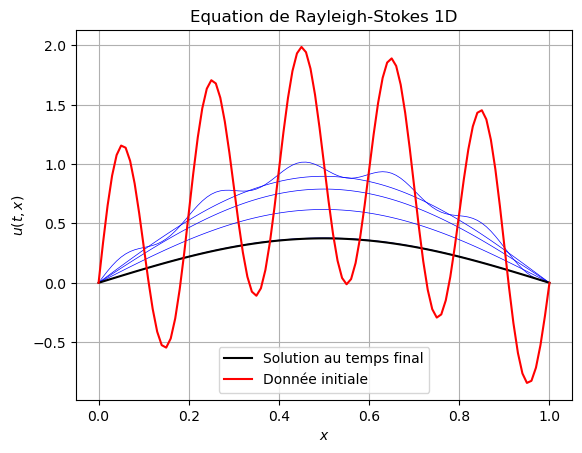
\includegraphics[width=\textwidth]{images/stabilité/alpha_dix_moins_5.png}
        \caption{$\alpha=10^{-5}$}
    \end{subfigure}
    \hfill
    \begin{subfigure}{0.32\textwidth}
        \centering
        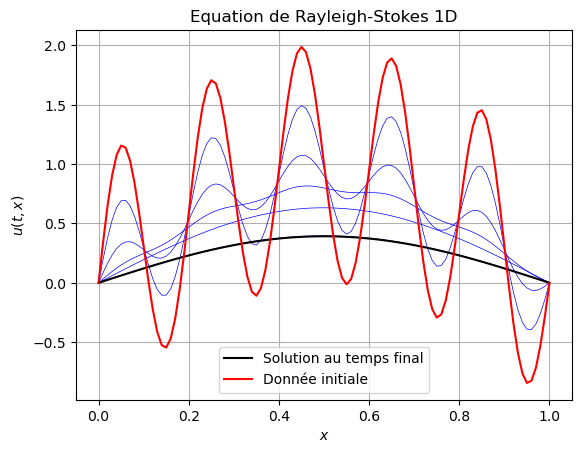
\includegraphics[width=\textwidth]{images/stabilité/alpha_dix_moins_2.png}
        \caption{$\alpha=5\times 10^{-3}$}
    \end{subfigure}
    \hfill
    \begin{subfigure}{0.32\textwidth}
        \centering
        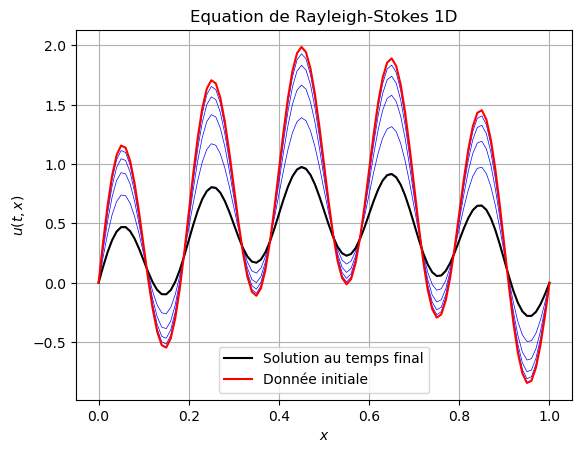
\includegraphics[width=\textwidth]{images/stabilité/alpha_dix_moins_1.png}
        \caption{$\alpha=10^{-1}$}
    \end{subfigure}
    \caption{Comportement des hautes fréquences en fonction de $\alpha$}
    \label{fig:stabilite_alpha}
\end{figure}
\end{frame}

\subsection{Un exemple}

%\begin{frame}{Créneau}
%\begin{itemize}
%\item On veut observer l'effet de régularisation de l'équation pour une donnée
%initiale discontinue.
%\item On s’intéresse donc au problème suivant
%   \begin{equation*}
%        \begin{cases}
%            \partial_tu(t,x) - \nu\partial_{xx} u(t,x) - \alpha\partial_{xx} \big(\partial_t u(t,x)\big) = 0 & \forall (t,x) \in \ ]0, T[ \ \times \ ]0,L[  \\
%            u(0,x) = u_0(x) = \mathds{1}_{\left[\tfrac{L}{4},\tfrac{3L}{4}\right]}(x) & \forall x \in \ ]0,L[ \\
%            u(t, 0) = u(t,L) = 0 & \forall t \in \ ]0,T[
%        \end{cases}
%    \end{equation*}
%    \item On résout numériquement le problème en posant 
%    $N = 200$, $L=10$ et $T=20$. Pour les paramètre de 
%    l'équation de Rayleigh-Stokes on choisi $\nu = 0.4$ et 
%    $\alpha=0.5$ Cela va nous permettre d'étudier 
%    comment varie notre solution initial et quels sont les 
%    effets du paramètre $\alpha$.
%    \end{itemize}
%\end{frame}

%\begin{frame}{Créneau}  
%\begin{figure}[!ht]
%        \centering
%        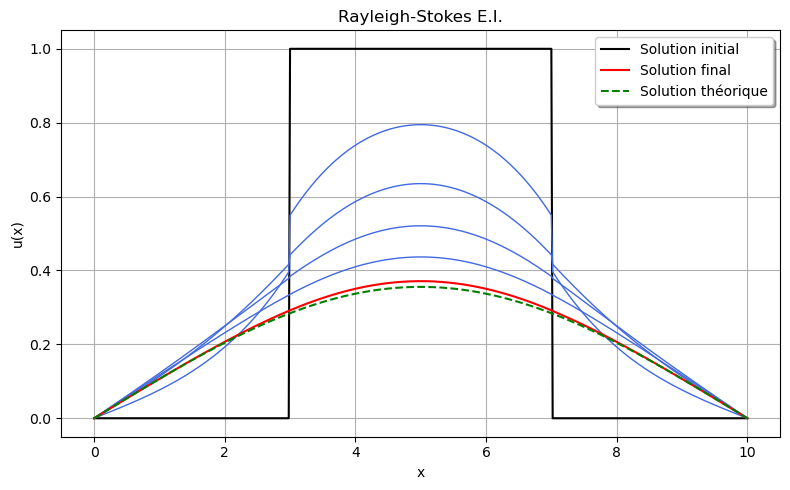
\includegraphics[width=0.6\textwidth]{images/Exemples/Indicatrice/resolution_indicatrice.png}
%    \caption{ Résolution de l'équation de Rayleigh-Stokes $1$D}
%    \label{fig:Exemples_RS_Stokes_indicatrice}
%\end{figure}
%\begin{eqnarray*}
%    u(t,x) = \sum_{k=1}^{N} \frac{2}{k\pi}\left(\cos\Big(\frac{k\pi}{4}\Big) -\cos\Big(\frac{3k\pi}{4}\Big)\right) \exp\left(-\frac{\nu\lambda_k}{1+\alpha\lambda_k}\,t\right)\sin\left(\frac{k\pi x}{L}\right)
%\end{eqnarray*}
%\end{frame}

%\begin{frame}
%    \begin{figure}[!ht]
%        \centering
%    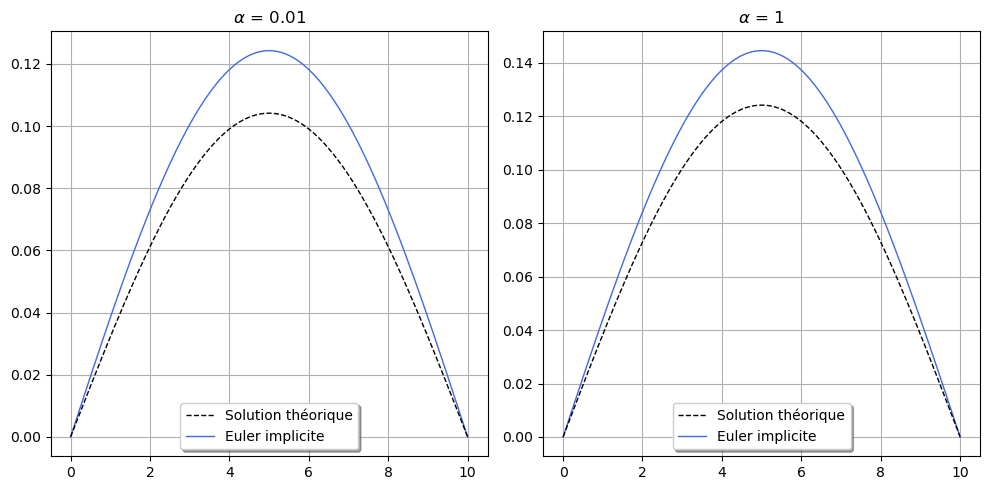
\includegraphics[width=\linewidth]{images/Exemples/Indicatrice/comparaison alpha indicatrice.png}
%    \caption{Comparaison en fonction de $\alpha$}
%    \label{Indicatrice_comparaisons des alpha}
%    \end{figure}
%\end{frame}

\begin{frame}{Problème de Stokes impulsif}
    \begin{itemize}
        \item On va maintenant simuler la réponse d'un fluide à l'accélération 
d'une paroi. 
\item Le problème s'écrit
\begin{equation*}
    \begin{cases}
        \partial_tu(t,x) - \nu\partial_{xx} u(t,x) - \alpha\partial_{xx} \big(\partial_t u(t,x)\big) = 0 & \forall (t,x) \in \ ]0, 5[ \ \times \ ]0,1[  \\
        u(0,x) = u_0(x) = 0 & \forall x \in \ ]0,1[ \\
        u(t,1) = 0 & \forall t \in \ ]0,5[ \\
        u(t,0) = U_0:=10 & \forall t \in \ ]0,5[
    \end{cases}
\end{equation*}
    \end{itemize}
\end{frame}

\begin{frame}{Problème de Stokes impulsif}
    \begin{figure}[!ht]
    \centering
    \begin{subfigure}{0.32\textwidth}
        \centering
        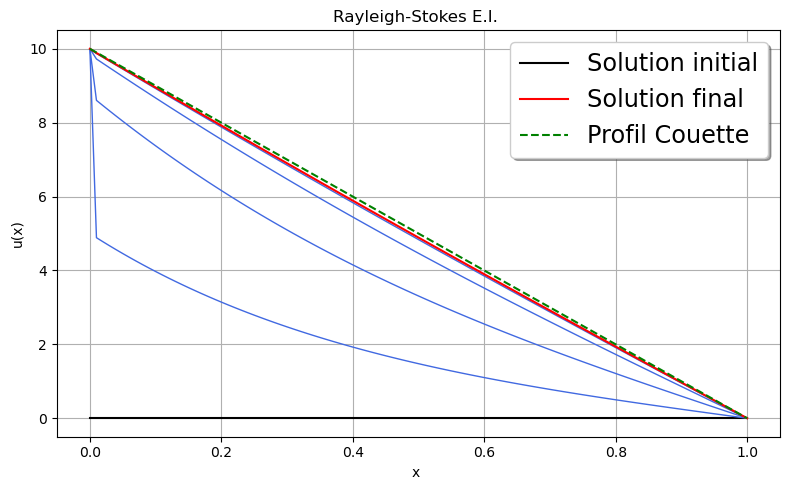
\includegraphics[width=\textwidth]{images/Exemples/Plaque en mouvement/RS_EI_plaque_1.png}
        \caption{$\alpha=0.1$}
    \end{subfigure}
    \hfill
    \begin{subfigure}{0.32\textwidth}
        \centering
        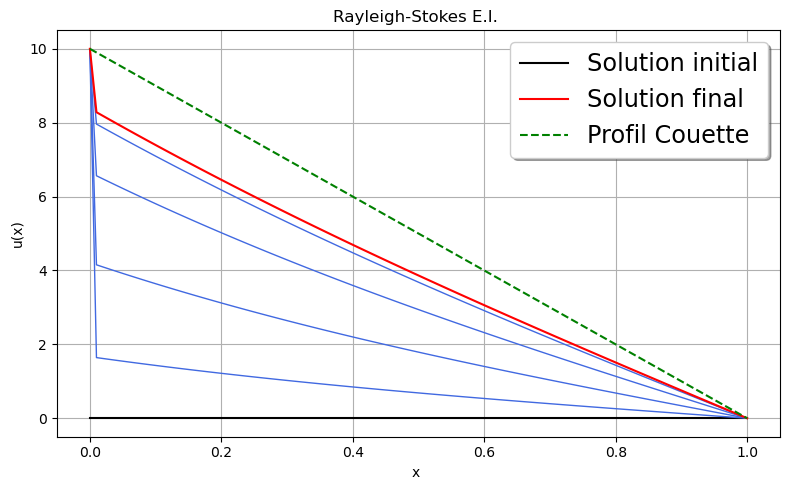
\includegraphics[width=\textwidth]{images/Exemples/Plaque en mouvement/RS_EI_plaque_2.png}
        \caption{$\alpha=0.5$}
    \end{subfigure}
    \hfill
    \begin{subfigure}{0.32\textwidth}
        \centering
        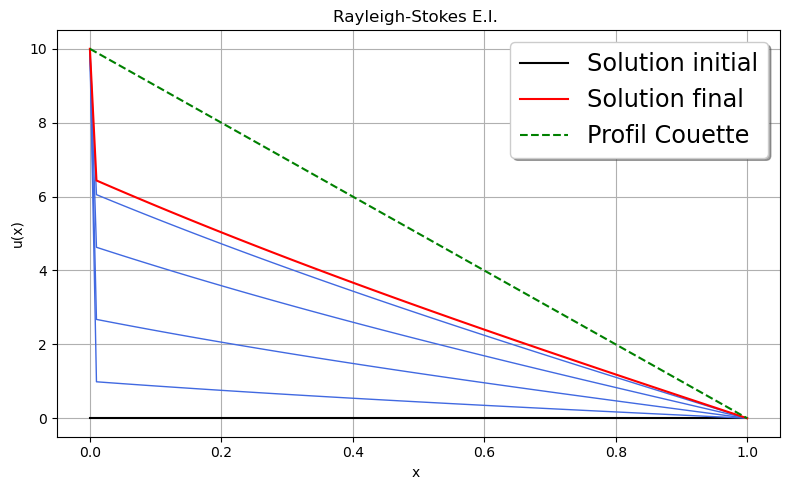
\includegraphics[width=\textwidth]{images/Exemples/Plaque en mouvement/RS_EI_plaque_3.png}
        \caption{$\alpha=0.9$}
    \end{subfigure}
    \caption{Influence du paramètre $\alpha$ sur la résistance du fluide face à la condition initiale pour l'équation de Rayleigh-Stokes $1$D}
    \label{fig:Exemples_RS_Stokes_impulsif}
\end{figure}
\end{frame}

\subsection{Comparaison avec l'équation de la chaleur}

\begin{frame}
    \begin{itemize}
    \item Problème aux limites pour l'équation de Rayleigh-Stokes
    \begin{equation*}
        \begin{cases}
            \partial_tu(t,x) - \nu\partial_{xx} u(t,x) - \alpha\partial_{xx} \big(\partial_t u(t,x)\big) = 0 & \forall (t,x) \in \ ]0, 1[ \ \times \ ]0,1[  \\
            u(0,x) = u_0(x) = \sin{(\pi x)} & \forall x \in \ ]0,1[ \\
            u(t, 0) = u(t,1) = 0 & \forall t \in \ ]0,1[
        \end{cases}
    \end{equation*}
    \item Problème aux limites pour l'équation de la chaleur
    \begin{equation*}
        \begin{cases}
            \partial_tu(t,x) - \nu\partial_{xx} u(t,x) = 0 & \forall (t,x) \in \ ]0,1[ \ \times \ ]0,1[  \\
            u(0,x) = u_0(x)=\sin{(\pi x)} & \forall x \in \ ]0,1[ \\
            u(t, 0) = u(t,1) = 0 & \forall t \in \ ]0,1[
        \end{cases}
    \end{equation*} 
    \item Les solutions de ces problèmes sont 
    \begin{eqnarray*}
        u_{\text{RS}}(t,x) = \sin{(\pi x)}\exp{\Big( -\frac{\nu \pi^2}{1+\alpha \pi^2}t\Big)}
        &\text{ et }& u_{\text{chal}}(t,x) = \sin{(\pi x)}\exp{(-\nu \pi^2t)}
    \end{eqnarray*}
\end{itemize}
\end{frame}

\begin{frame}
    \begin{itemize}
        \item L'objectif ici est d'observer l'influence du paramètre $\alpha$ sur la dissipation de l'énergie cinétique et de comparer ce phénomène avec l'équation de la chaleur (cas $\alpha=0$). 
        \item Pour nos simulations, on choisit $\nu = 0.1$, et $h=\Delta t = \dfrac{1}{100}$. La simulation pour l'équation de la chaleur donne le résultat suivant
\begin{figure}[!ht]
    \centering
    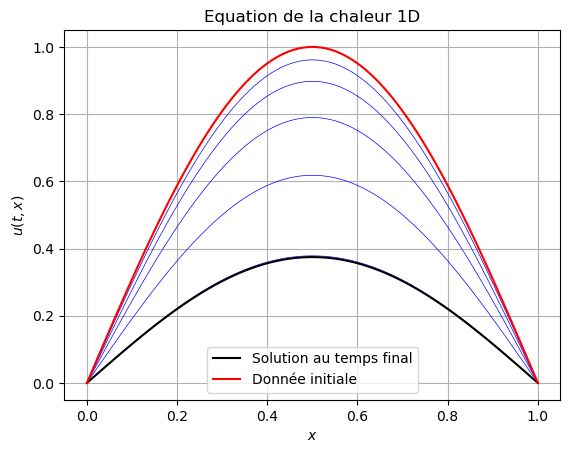
\includegraphics[width=0.5\linewidth]{images/comparaison_chaleur/eq_chaleur.png}
    \caption{\'Equation de la chaleur $1$D pour l'évolution temporelle du profil de vitesse $u(t,x)$ pour un mode sinusoïdal}
    \label{fig:eqchaleur}
\end{figure}
    \end{itemize}
\end{frame}

\begin{frame}
    \begin{itemize}
        \item Pour comparer à l'équation de Rayleigh-Stokes, on choisit $\alpha \in \{5\times 10^{-1}, 5 \times 10^{-2}, 5 \times 10^{-4}\}$. 
    \end{itemize}
        \begin{figure}[!ht]
    \centering
    \begin{subfigure}{0.32\textwidth}
        \centering
        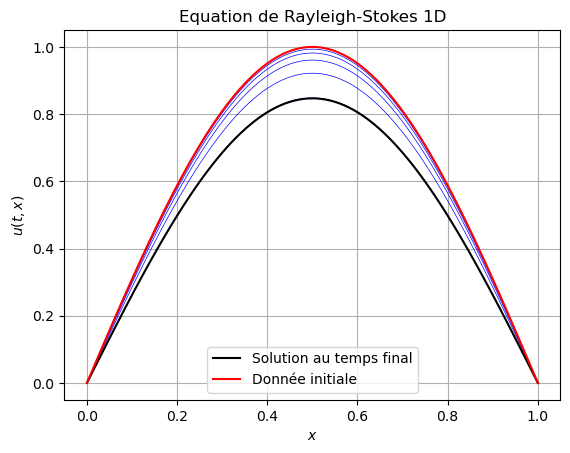
\includegraphics[width=\textwidth]{images/comparaison_chaleur/eq_RS_alpha1.png}
        \caption{$\alpha=5\times 10^{-1}$}
    \end{subfigure}
    \hfill
    \begin{subfigure}{0.32\textwidth}
        \centering
        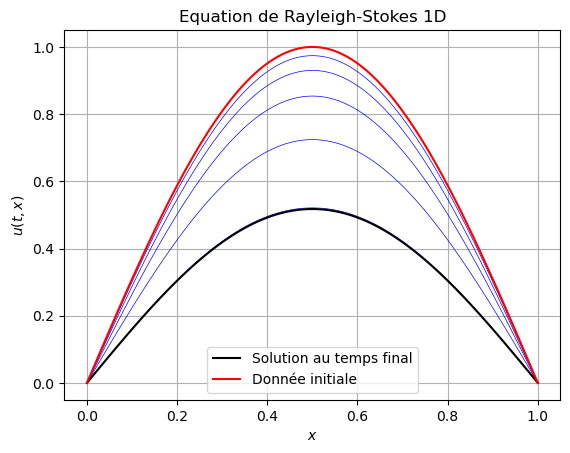
\includegraphics[width=\textwidth]{images/comparaison_chaleur/eq_RS_alpha2.png}
        \caption{$\alpha=5\times 10^{-2}$}
    \end{subfigure}
    \hfill
    \begin{subfigure}{0.32\textwidth}
        \centering
        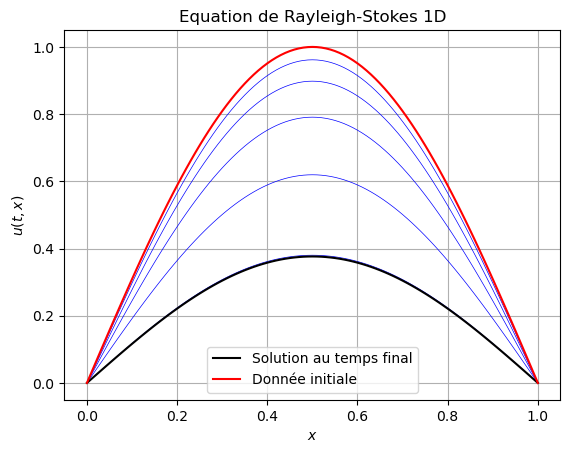
\includegraphics[width=\textwidth]{images/comparaison_chaleur/eq_RS_alpha3.png}
        \caption{$\alpha=5 \times 10^{-4}$}
    \end{subfigure}
    \caption{Influence du paramètre $\alpha$ sur la dissipation de l'énergie pour l'équation de Rayleigh-Stokes $1$D}
    \label{fig:comparaisonchaleurRS}
\end{figure}
\end{frame}

%\begin{frame}{Code C++}
%    \begin{figure}[!ht]
%    \centering
%    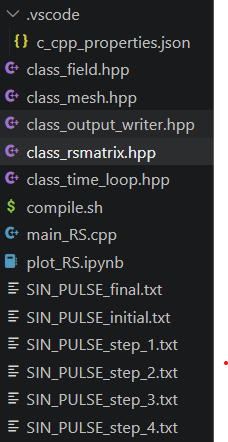
\includegraphics[width=0.25\linewidth]{images/code.png}
%    \caption{Architecture du code C++}
%    \label{fig:code}
%\end{figure}
%\end{frame}

\section{Approximation par la méthode Galerkin discontinu}
\begin{frame}
\begin{itemize}
    \item  Fait un lien entre les méthodes de volumes finis et d'éléments finis. \\
    Recherche de la formulation variationnelle puis on cherche la solution discrète.
    \item Cependant grande différence avec ces méthodes, aucune continuité n’est imposée aux interfaces entre les éléments du maillage.
\end{itemize}
   
\begin{figure}
    \centering
    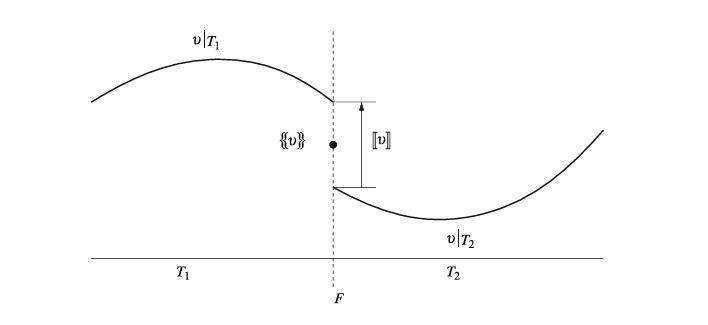
\includegraphics[width=0.5\linewidth]{images/Galerkine_Discontinue/image_maille_GD.JPG}
    \caption{Exemple d'une façon de gérer le flux au niveau de l'intervalle.}
    \label{flux_GD_exemple}
\end{figure}
\begin{equation*}
    \{\!\!\{v\}\!\!\}_F(x) := \tfrac{1}{2}\left(v|_{T_1}(x)+v|_{T_2}(x)\right) \ \ \ \ \ \ \ \ [\![v]\!] := v|_{T_1}(x)-v|_{T_2}(x)
\end{equation*}

\end{frame}

\begin{frame}{Réécrire le problème}
\begin{itemize}
\item On commence par partir du problème de Rayleigh-Stokes $1$D homogène
\begin{equation*}
    \begin{cases}
        \partial_tu(t,x) - \nu\partial_{xx} u(t,x) - \alpha\partial_{txx} u(t,x) = 0 & (t,x) \in \mathbb R_+ \times \bbR  \\
        u(0,x) = u_0(x) & x \in \bbR
    \end{cases}
\end{equation*}  
\item Puis en faisant comme en élément fini, on se retrouve en $1D$ avec:
\begin{equation*}
    \int_{K_i} \partial_t uv + \nu \int_{K_i}\partial_{x}u\partial_{x}v \ + \alpha \int_{K_i} \partial_{tx}u\partial_{x}v
    =  \nu \Big[\partial_{x}u v \Big]^{x_i +h/2}_{x_i - h/2} \ + \alpha \Big[\partial_{tx}u v \Big]^{x_i +h/2}_{x_i - h/2} 
\end{equation*}
\item Le choix de la base change le problème. Prenons la base $\{e_0\} = \{1\}$.
\begin{equation*}
    \partial_x u_h\big|_{x_i + h/2} = \frac{u_0^{i+1} - u_0^i}{h}, \qquad
    \partial_x u_h\big|_{x_i - h/2} = \frac{u_0^i - u_0^{i-1}}{h}
\end{equation*}
\begin{equation*}
    h\,\partial_t u_0^i = \frac{\nu}{h}\left(u_0^{i+1} - 2u_0^i + u_0^{i-1}\right)
    + \frac{\alpha}{h}\left(\partial_t u_0^{i+1} - 2\partial_t u_0^i + \partial_t u_0^{i-1}\right)
\end{equation*}
\end{itemize}
\end{frame}

\begin{frame}{Le cas P1}
Pour $j$ valant $0$ ou $1$ on obtient le système suivant:
\begin{eqnarray*}\label{EDP_RS_Formulation_Faible_P1}
  &\partial_t u_i^0 \displaystyle{\int_{K_i}}  \phi_0 \phi_j + \partial_t u_i^1 \displaystyle{\int_{K_i}}   \phi_1 \phi_j& \\
   &+\nu \ u_i^0  \displaystyle{\int_{K_i}} \partial_{x}\phi_0 \partial_{x}\phi_j  + \nu \ u_i^1 \displaystyle{\int_{K_i}} \partial_{x}\phi_1 \partial_{x}\phi_j& \\
   &+ \alpha \partial_{t}u_i^0 \displaystyle{\int_{K_i}}  \partial_{x}\phi_0\partial_{x}\phi_j + \alpha \partial_{t}u_i^1 \displaystyle{\int_{K_i}}  \partial_{x}\phi_1\partial_{x}\phi_j &\\
    &=& \\ 
    &\nu \Big[\partial_{x}\big(u_i^0\phi_0 +u_i^1\phi_1 \big) \phi_j  \Big]^{x_i +h/2}_{x_i - h/2} \ + \alpha \Big[\partial_{tx}\big(u_i^0\phi_0 +u_i^1\phi_1 \big) \phi_j \Big]^{x_i +h/2}_{x_i - h/2} 
\end{eqnarray*}
Ce qui en calculant les matrices de rigidité et de masse donne:
\begin{eqnarray*}
    &&\begin{bmatrix}
        h & 0 \\
        0 & \frac{h}{12} 
    \end{bmatrix}
    \begin{bmatrix}
    \partial_t u_i^0 \\
    \partial_t u_i^1    
    \end{bmatrix}
    +
        \begin{bmatrix}
        0 & 0 \\
        0 & \frac{\nu + \alpha \partial_t}{h} 
    \end{bmatrix}
    \begin{bmatrix}
    u_i^0 \\
    u_i^1    
    \end{bmatrix}
    = (\nu + \alpha\partial_t)
    \begin{bmatrix}
    \{\!\!\{ u_i^1 \}\!\!\}_{F_i} - \{\!\!\{ u_i^1 \}\!\!\}_{F_{i-1}}\\
    \{\!\!\{ u_i^1 \}\!\!\}_{F_i} \times\frac{1}{2} - \{\!\!\{ u_i^1 \}\!\!\}_{F_{i-1}} \times (- \frac{1}{2})
    \end{bmatrix} \\
\end{eqnarray*}
\end{frame}

\begin{frame}
    \begin{itemize}
        \item Les problèmes de second grade doivent traiter de façon plus subtile le flux numérique.
        \item La méthode reste naturelle pour traiter ce genre de problème. Le terme $\alpha$ permet de régulariser les phénomènes de chocs qui entraînent une diffusion numérique pour cette méthode.
    \end{itemize}
\end{frame}


\begin{frame}
    \begin{center}
        \Large Merci pour votre écoute !
    \end{center}
\end{frame}

\end{document}